\documentclass[twoside,english]{uiofysmaster}
%\bibliography{references}

\usepackage{array}
\usepackage{booktabs}
\usepackage{float}
\usepackage{scrextend}
\usepackage{amsfonts}
\usepackage{amsmath,amsfonts,amssymb}
\addtokomafont{labelinglabel}{\sffamily}

\usepackage[boxed]{algorithm2e}
\addtokomafont{labelinglabel}{\sffamily}

% Feynman slash
\usepackage{slashed}

% To show code
\usepackage{listings}

% For quotes
\usepackage[autostyle]{csquotes} 

\setlength{\heavyrulewidth}{1.5pt}
\setlength{\abovetopsep}{4pt}

\begin{document}

\tableofcontents



\chapter{Gaussian Processes}

In this chapter Gaussian process regression is introduced and explained. To begin with some concepts and expressions in Bayesian statistics are introduced. The following section introduces the mathematical framework needed, before some covariance functions are discussed. A few concepts in Bayesian model selection are used as a basis to quantify the quality of predictions. Finally, distributed Gaussian processes are introduced as a way of scaling Gaussian processes to larger datasets.

\section{Introduction to Bayesian Statistics}

As it turns out, statistics are not merely statistics. In fact, there is great disagreement as to what statistics should be. The main opponents in this fight can be divided into two groups: the \textit{frequenstist} statisticians and the \textit{Bayesian} statisticians. In order to understand why they can't get along, first consider a statement they \textit{do} agree on

\begin{center}
\textit{Statisticians use probability to describe uncertainty.}
\end{center}

This seems reasonable. Where statisticians reach disagreement is at the definition of the \textit{uncertain}. Defining the uncertain defines probability, and at a high level one can distinguish between two branches, namely \textit{objective} and \textit{subjective} probability. Consider an example in which a statistician throws a dice. Before throwing, he is uncertain about the outcome of the dice toss. This uncertainty related to the outcome is the \textit{objective uncertainty}: no one can know if he will throw a 1 or a 4. On the other hand, he might also be uncertain about the underlying probability distribution of the dice toss. Is the dice loaded? Is one of the edges sharper than the others? This uncertainty is the \textit{subjective uncertainty}, as it may vary from person to person depending on how much information one has about the system. One of the main critiques of subjective probability posed by frequentists is that the final probability depends on who you ask.

\subsection{Bayes' Theorem}

To further illustrate the difference it is helpful to introduce a soundingly Bayesian framework, namely \textit{Bayes' theorem}. Bayes' theorem can be derived from the familiar rules of probability
\begin{align}\label{Eq:: Sum rule}
P(X | I) + P(\bar{X} | I) = 1,
\end{align}
\begin{align}\label{Eq:: Product rule}
P(X, Y | I) = P(X | Y, I) \times P(Y | I),
\end{align} 
commonly known as the \textit{sum rule} and \textit{product rule}, respectively. $P(X|I)$ means the probability of outcome $X$ given the information $I$, and $P(X|Y,I)$ means the probability of outcome $X$ given the information $I$ \textit{and} outcome $Y$. The bar over $\bar{X}$ means that the outcome $X$ does \textit{not} happen. The sum rule states that the probability of the outcome $X$ happening plus the probability of $X$ not happening is equal to 1. This is rather untuitive, considering an event either takes place or it doesn't. The second rule, the product rule, states that the probability of both outcomes $X$ and $Y$ is equal to the probability of $Y$ times the probability of $X$ given that $Y$ has already happened. 
These expressions can easily be combined into Bayes' theorem, first formulated by reverend Thomas Bayes in 1763,
\begin{align}\label{Eq:: gaussian process : Bayes theorem}
P(X | Y, I) = \frac{P(Y | X, I) \times P(X | I)}{P(Y | I)}.
\end{align}
This theorem states that the probability of $X$ given $Y$ equals the probability of $Y$ given $X$ times the probability of $X$, divided by the probability of $Y$. So what is Bayesian about Bayes' theorem? \textit{Nothing}. It merely reformulates the rules of logical consistent reasoning statet by Richard Cox in 1946 \cite{sivia2006data}. Laplace was the one to make Bayes' theorem Bayesian, when he used the theorem to perform inference about distribution parameters. These are, for example, the mean and variance of a Gaussian distribution. The resulting expression is
\begin{align}
P(\Theta = \theta | X=x) = \frac{P(X=x|\Theta = \theta) P(\Theta = \theta)}{P(X=x)},\label{Eq:: gaussian process : Bayesian inference}
\end{align}
where $\Theta$ are the possible probability distribution parameters, $X$ are the possible outcomes, $P(X=x)$ is a normalization constant called the \textit{marginal likelihood}, and $P(X=x|\Theta = \theta)$  and $P(\Theta = \theta)$ are the \textit{likelihood} and \textit{prior}, respectively, both of which will be revisited later. In other words, Eq. (\ref{Eq:: gaussian process : Bayesian inference}) states the probability of the parameters $\theta$, given the knowledge of outcomes $x$.

A crucial parting of the Bayesians from the frequentists is at the introduction of the \textit{prior}, which expresses a probability distribution on the \textit{parameters} of the probability distribution. Fret not, this will be further explained.

\subsection{Priors and Likelihood}

The likelihood $P(X = x |\Theta = \theta)$ is simply the probability of the observations given the parameters. This is rather intuitive, the more interesting concept introduced is the prior. The prior expresses belief or assumption of the data, and has to be determined beforehand. By using Bayes' theorem in the version from Eq. (\ref{Eq:: gaussian process : Bayesian inference}), we end up with the measure $P(\Theta = \theta | X = x)$, also called the \textit{posterior distribution}. This can be thought of as our prior belief, modified by how well this belief fits the data obtained,
\begin{align*}
\text{posterior} = \frac{\text{prior} \times \text{likelihood}}{\text{marginal likelihood}}.
\end{align*}
Consider an example. The statistician from before has now grown tired of throwing dice, and starts to throw a coin. Before the throw he assumes the probability of getting heads or tails is equal, so he assumes a flat prior. After one throw he gets heads, and the posterior changes to a function with high probability for heads, and low for tails. Another heads makes the posterior even narrower around 1, but after several throws the distribution converges to a narrow peak around $0.25$, as can be seen in Fig. (\ref{Fig:: gaussian process : Dice throw }), along with other examples of priors. This indicates an unfair coin. Note that the different priors arrive at the same posterior after a large amount of throws

\begin{figure}
\centering
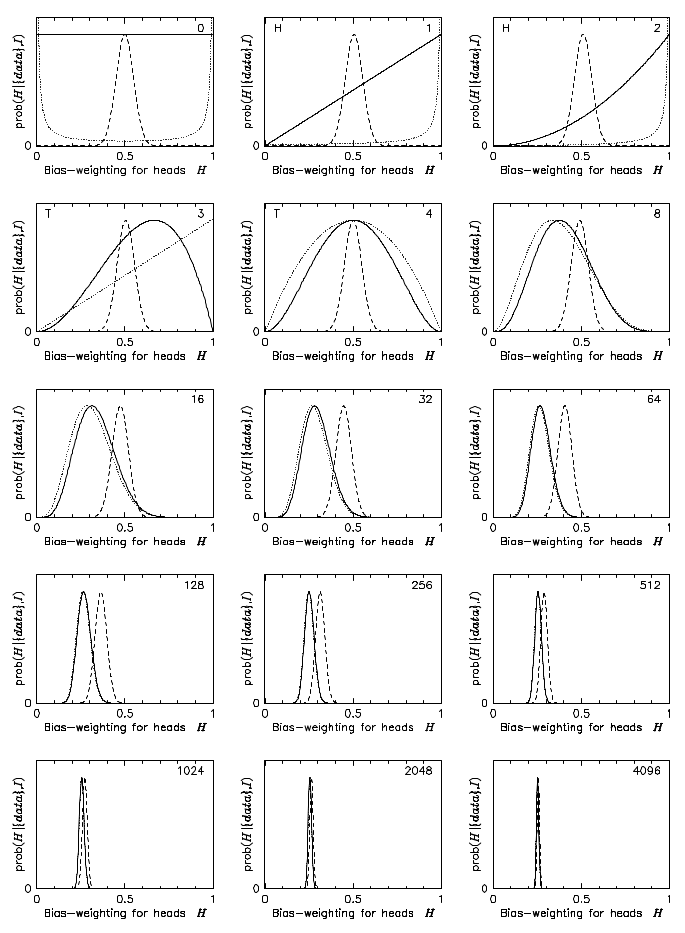
\includegraphics[scale=0.65]{sivia_coin_toss.png}
\caption{The effect of different priors, $P(H|I)$, on the posterior pdf for the bias-weighting of a coin. The solid line is a flat prior, the dashed line assumes a fair coin, and the dotted line is the Jeffreys prior. Figure from \cite{sivia2006data}.}
\label{Fig:: gaussian process : Dice throw }
\end{figure}


\subsection{Best Estimate and Reliability}

Now that the posterior distribution has been defined, it would be useful with a way to quantify how well it actually fits the data. For that purpose the \textit{best estimate} and \textit{reliability} are introduced. The best estimate $X_0$  is the outcome with the highest probability. In other words, it is the maximum of the posterior
\begin{align}
&\frac{dP}{dX}\Big|_{X_0} = 0, &\frac{d^2P}{dX^2}\Big|_{X_0} < 0.
\end{align}
The second derivative must be negative in order to insure that it is, in fact, a maximum. Once the best estimate has been found, one should ask oneself how reliable this estimate is. This reliability is represented by the width of the distribution. A very narrow distribution has very low uncertainty, while a wide distribution has a higher probability for the values aroung the best estimate. The width is found using a Taylor expansion of the posterior, and taking the logarithm \footnote{$L$ is a monotonic function of $P$, so the maximum of $L$ is at the maximum of $P$.}
\begin{align}
&L = L(X_0) + \frac{1}{2} \frac{d^2}{dx^2} L\Big|_{X_0} (X-X_0)^2 +... ,&L = \log_e \Big[\text{prob}(x | \{data\}, I) \Big]\label{Eq:: gaussian process : Taylor expansion L}
\end{align}
This gives a proximate posterior which is a \textbf{Gaussian distribution}, with mean and variance given by
\begin{align}
&\text{prob}(x| \mu, \sigma) \text{ where } \mu = X_0\text{, } \sigma = \Big( - \frac{d^2L}{dx^2} \Big)^{-1/2}.
\end{align}
The Gaussian distribution is symmetric with respect to the maximum at $x = \mu$, and has a full width at half maximum (FWHM) at around $2.35 \sigma$, as shown in Fig. (\ref{Fig:: gaussian process : Gaussian distribution}).

\begin{figure}
\centering
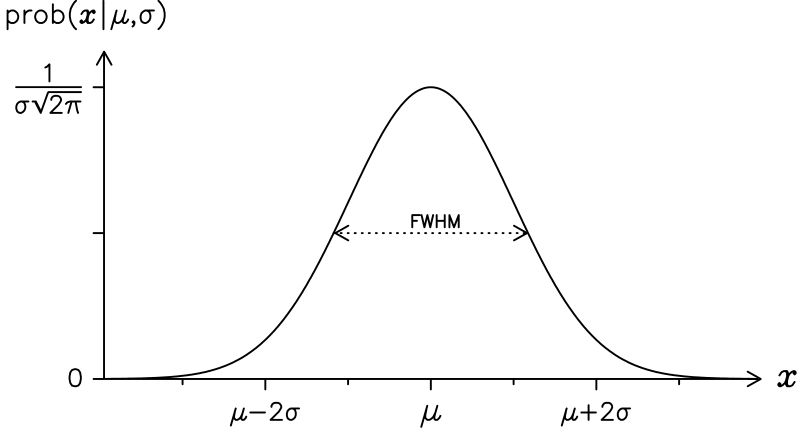
\includegraphics[scale=0.5]{sivia_gaussian_distribution.png}
\caption{A Gaussian probability distribution. The maximum is at the mean value $\mu$, with a full width at half maximum (FWHM) at around $2.35 \sigma$. Figure from \cite{sivia2006data}.}
\label{Fig:: gaussian process : Gaussian distribution}
\end{figure}

\subsection{Covariance}

The final term needed before embarking on Gaussian processes is \textit{covariance}. In most cases the expressions one has to solve are not as simple as Eq. (\ref{Eq:: gaussian process : Taylor expansion L}), as the probability distribution will normally have several quantities of interest $\{ X_i \}$. In that case, one has to solve a set of \textit{simultaneous equations} in order to get the best estimate
\begin{align}\label{Eq:: gaussian process : Best estimate X_i}
\frac{dP}{dX_i} \Big|_{X_{0j}} =0,
\end{align}
This section is discussed in more detail in \cite{sivia2006data}. In order to get simpler expressions, consider the problem in two dimensions, so that $\{ X_i \} = (X, Y)$. The Taylor expansion of $L$ is then
\begin{align}\label{Eq:: gaussian process : Taylor expansion L_i}
L =& L(X_0, Y_0) + \frac{1}{2} \Big[ \frac{d^2L}{dX^2}  \Big|_{X_0, Y_0}(X-X_0)^2 \nonumber \\
& + \frac{d^2L}{dY^2}  \Big|_{X_0, Y_0}(Y-Y_0)^2 + 2 \frac{d^2L}{dXdY}  \Big|_{X_0, Y_0}(X-X_0)(Y-Y_0) \Big] +...
\end{align}
There are now four partial derivatives, reduced to three using the rules for mixed partial derivatives $\frac{\partial^2}{\partial X \partial Y} = \frac{\partial^2}{\partial Y \partial X}$. Writing the quadratic part of \ref{Eq:: gaussian process : Taylor expansion L_i} in matrix form gives
\begin{align}
Q = 
\begin{pmatrix}
X-X_0 & Y -Y_0
\end{pmatrix}
\begin{pmatrix}
A & C\\
C & B
\end{pmatrix}
\begin{pmatrix}
X -X_0\\
Y-Y_0
\end{pmatrix},
\end{align}
where the matrix elements are
\begin{align}
&A = \frac{\partial^2 L}{\partial X^2} \Big|_{X_0, Y_0}, &B = \frac{\partial^2 L}{\partial Y^2} \Big|_{X_0, Y_0}, &&C = \frac{\partial^2 L}{\partial X \partial Y} \Big|_{X_0, Y_0}.
\end{align}
On a seemingly unrelated note, we define the \textit{variance} as the expectation value of the square of deviations from the mean. In the two-dimensional case this becomes \cite{sivia2006data}
\begin{align}
\text{Var}(X) = \sigma_x^2 = \braket{(X - X_0)^2} = \int \int (X - X_0)^2 P (X, Y | \{\text{data}\}, I) dXdY.
\end{align}
This quantity is called the variance $\sigma_X^2$, and its square root is the standard deviation $\sigma_X$. A similar expression can be found for $Y$, by switching $X$ and $Y$. It is also possible to find the simultaneous deviations of the parameters $X$ and $Y$, or the correlation between the inferred parameters. This is called the \textit{covariance} $\sigma_{XY}^2$, and is in this case
\begin{align}
\sigma_{XY}^2 = \braket{(X - X_0) (Y - Y_0)} =\int \int (X - X_0) (Y - Y_0) P (X, Y | \{\text{data}\}, I) dXdY.
\end{align}
The covariance indicates how an over- or underestimation of one parameter affects the other parameter. If, for example, an overestimation of $X$ leads to an overestimation of $Y$, the covariance is positive. If the overestimation of $X$ has little or no effect on the estimation of $Y$, the covariance is negligible or zero $|\sigma_{XY}| \ll \sqrt{\sigma_X^2 \sigma_Y^2}$. These effects are illustrated in Fig. (\ref{Fig:: gaussian process : Covariance illustrated}). It can be shown that \cite{sivia2006data}
\begin{align}
\text{cov} = 
\begin{pmatrix}
\sigma_X^2 & \sigma_{XY}^2\\
\sigma_{XY}^2 & \sigma_Y^2
\end{pmatrix}
= - \begin{pmatrix}
A & C\\
C & B
\end{pmatrix}^{-1}.
\end{align}
This is called the \textit{covariance matrix}.

\begin{figure}
\centering
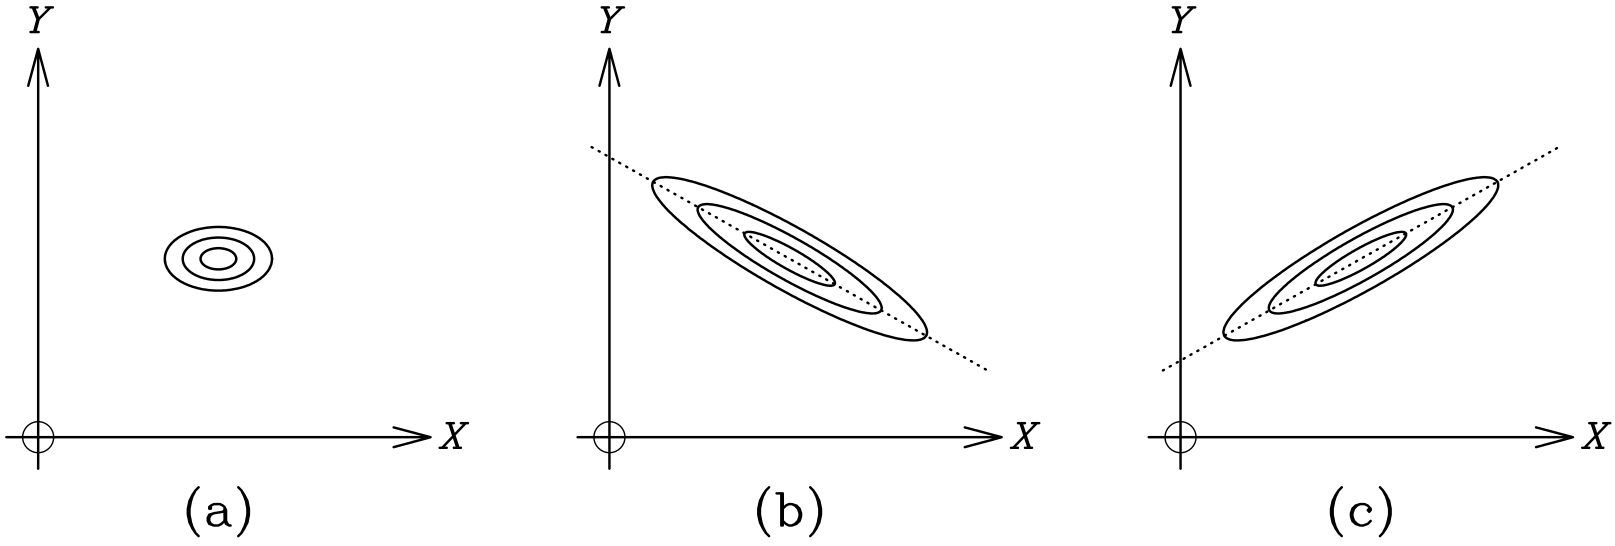
\includegraphics[scale=0.25]{sivia_covariance_correlation.png}
\caption{A schematic illustration of covariance and correlation. (a) The contours of a posterior pdf with zero covariance, where the inferred values of $X$ and $Y$ are uncorrelated. (b) The corresponding plot when the covariance is large and negative; $Y + mX =$ constant along the dotted line (where $m > 0$), emphasizing that only this sum of the two parameters can be inferred reliably. (c) The case of positive correlation, where we learn most about the difference $Y − mX$; this is constant along the dotted line. Figure from \cite{sivia2006data}}
\label{Fig:: gaussian process : Covariance illustrated}
\end{figure}

\pagebreak


\section{Gaussian Process Regression}

\begin{figure}[H]
\centering
\includegraphics[scale=0.15]{gp_title.jpg}
\end{figure}


Now that some basics of Bayesian statistics and Gaussian distributions have been covered, it's time to delve into the subject of Gaussian Processes. Gaussian processes are a supervised machine learning method, designed to solve regression and probabilistic classification problems. In this thesis the focus will be solely on regression problems. As experience dictates that Gaussian Processes can be somewhat hard to grasp, it will serve both the reader and the author well to begin on a conceptual level: \textit{what do Gaussian Processes do?}

Consider a set of points $\{x_i\}, \{f(x_i)\}$, such as the blue dots shown in Fig. (\ref{Fig:: gaussian process : GP illustration}). The set of points is discrete, and so imagine that the value $f(x^*)$ for some $x^*$ is unknown. Gaussian Processes (GP) finds a distribution \textit{of function values} at this point $x^*$. This ditribution is Gaussian, and its mean is the value $f^*$ predicted by the GP. The variance of the distribution $\sigma^2$ is the uncertainty of this value, as illustrated by the Gaussian distribution in the point $x^*$ in Fig. (\ref{Fig:: gaussian process : GP illustration}). So Gaussian Processes provide a \textit{distribution over function values}, meaning that for each $x$ one can find a Gaussian distribution over $f(x)$ with a mean value $\mu \simeq f(x)$ and an uncertainty $\sigma$. 

\begin{figure}
\centering
\includegraphics[scale=0.25]{gaussian_process_illustration.jpg}
\caption{An illustration of a Gaussian Process prediction of the function value $f(x^*)$ (blue cross) given the known set of points $\{x_i, f(x_i)\}$ (blue dots). The prediction is a Gaussian distribution in $f(x^*)$ with mean $f(x^*)$ and variance $\sigma^2$.}
\label{Fig:: gaussian process : GP illustration}
\end{figure}

The mean value of the distribution in $f(x^*)$ is a linear combination of the known function values $\{ f(x_i) \}$, weighted by the covariance between $x_i$ and the test value $x^*$. The covariance is decided by the \textit{kernel function}, which will be revisited. 

The more general framework considers multidimensional $\textbf{x}$, so that the set of known points, or \textit{training points}, are a matrix $\{X_i\}$. Input vectors are in machine learning called \textit{features}. The corresponding function values $y_i$ are called \textit{targets}. For a single point $\textbf{x}$ the mean  $m(\textbf{x})$ and covariance function $k(\textbf{x}, \textbf{x}')$ are defined as
\begin{align}
m(\textbf{x}) &= \mathbb{E}[f(\textbf{x})],\\
k(\textbf{x}, \textbf{x}') &= \mathbb{E} [(f(\textbf{x}) - m(\textbf{x}))(f(\textbf{x}') - m(\textbf{x}'))],
\end{align}
where $\mathbb{E}[y(\textbf{x})]$ is the expectation value of some function $y(\textbf{x})$. The mean and covariance define the Gaussian distribution for $f(\textbf{x})$, which is denoted 
\begin{align}
f(\textbf{x}) \sim \mathcal{GP}(m(\textbf{x}), k(\textbf{x}, \textbf{x}')).
\end{align}
The covariance $k(\textbf{x}_p, \textbf{x}_q)$ is thus decided by a covariance function, or a \textit{kernel}. The running example in this text with be the squared exponential (SE) kernel, given by
\begin{align}
k(f(\textbf{x}_p), f(\textbf{x}_q)) = k(\textbf{x}_p, \textbf{x}_q) = \exp \Big( - \frac{1}{2} |\textbf{x}_p - \textbf{x}_q|^2 \Big).
\end{align}
Note that the covariance of the function values $f(\textbf{x}_p)$, $f(\textbf{x}_q)$ only depends on the input parameters $\textbf{x}_p$, $\textbf{x}_q$. 

Specifying the covariance function implies a distribution over functions \cite{rasmussen2006gaussian}. This is because the allowed functions are now restricted to the set of functions that obey the correlation decided by $k(\textbf{x}_p, \textbf{x}_q)$. Using the kernel on a number of input points $X^*$ gives the covariance matrix, and giving an inital mean of zero provides the distribution
\begin{align}
f(x) \sim \mathcal{N} (0, K(X^*, X^*)).
\end{align} 
This is the \textit{prior} on the the function distribution. This distribution encodes the prior knowledge one has about the function values $f(x)$, and so the choice of kernel is one of the most important steps in learning with Gaussian Processes. This prior is modified by the training data to provide a posterior distribution. One can draw samples from both the prior and posterior, as shown in Fig. (\ref{Fig:: gaussian process : prior posterior drawn samples}).

\begin{figure}
\centering
\includegraphics[scale=0.4]{/home/ingrid/Documents/Master/Programs/Draw_Samples/draw_samples_benchmark.pdf}
\caption{Drawing functions from the prior (top) and posterior (bottom) distributions. The prior has mean 0 and covariance given by the squared exponential function. The posterior has been modified by training points (red dots), where the uncertainty is now zero, and the mean value is changed. Figure generated using scikit-learn.}
\label{Fig:: gaussian process : prior posterior drawn samples}
\end{figure}

To apply GP, consider a simple example of a noise-free set of training points $\{x_i, f(x_i)\}$. The joint distribution of training outputs, $\textbf{f}$, and test outputs, $\textbf{f}^*$, according to the prior is
\begin{align}
\begin{bmatrix}
\textbf{f}\\
\textbf{f}^*
\end{bmatrix}
\sim 
\mathcal{N} \Bigg(
\boldsymbol{0},
\begin{bmatrix}
K(X, X) & K(X, X^*)\\
K(X, X^*) & K(X^*, X^*)
\end{bmatrix}
 \Bigg)
\end{align}
For $n$ training points and $n^*$ test points, $K(X,X)$ is the $n \times n$ matrix containing the covariance of training points, $K(X, X^*)$ is the $n \times n^*$ matrix of covariance between the test and training points, and $K(X^*, X^*)$ is the $n^* \times n^*$ matrix containing the covariance of test points. By \textbf{conditioning} the distribution of $\textbf{f}^*$ on the observations,  one finds \cite{rasmussen2006gaussian} \footnote{For more details, see Appendix A.2 in \cite{rasmussen2006gaussian}.}
\begin{align}
\textbf{f}_* \big| X_*, X, \textbf{f} \sim \mathcal{N}&(K(X_*, X)K(X, X)^{-1} \textbf{f},\\ &K(X_*, X_*) - K(X_*, X)K(X, X)^{-1}K(X, X_*)).
\end{align}
Now one can draw samples from this distribution, as illustrated in Fig. (\ref{Fig:: gaussian process : prior posterior drawn samples}).


\subsection{Gaussian Noise Model}

In the real world, noise-free observations are very hard to come by. In most cases, the signal will contain some noise $y = f(\textbf{x}) + \varepsilon$, where the noise is assumed to follow a Gaussian distribution $\varepsilon \sim \mathcal{N}(0, \sigma_n^2)$. This is the \textit{Gaussian noise model}. The covariance can then be expressed as
\begin{align}
&\text{cov}(y_p, y_q) = k(\textbf{x}_p, \textbf{x}_q) + \sigma_n^2 \delta_{pq} &\text{cov}(\textbf{y}) = K(X, X) + \sigma_n^2 \mathbb{I}
\end{align}
The prior distribution is now
\begin{align}
\begin{bmatrix}
\textbf{y}\\
\textbf{f}_*
\end{bmatrix}
\sim 
\mathcal{N} \Bigg(
\boldsymbol{0},
\begin{bmatrix}
K(X, X) + \sigma_n^2 \mathbb{I} & K(X, X_*)\\
K(X, X_*) & K(X_*, X_*)
\end{bmatrix}
 \Bigg),
\end{align}
which gives for the conditioned distribution 
\begin{align}
\textbf{f}_* \big| X_*, X, \textbf{f} & \sim \mathcal{N}(\bar{\textbf{f}}_*, \text{cov}(\textbf{f}_*)), \text{ where}\\
\bar{\textbf{f}}_* &= K(X_*, X) [K(X, X) + \sigma_n^2 \mathbb{I}]^{-1} \textbf{y},\\
\text{cov} (\textbf{f}_*) &= K(X_*, X_*) - K(X_*, X)[K(X, X) + \sigma_n^2 \mathbb{I}]^{-1} K(X, X_*)
\end{align}

In order to tidy up the expression somewhat, define the matrix $K \equiv K(X, X)$ and the matrix $K_* = K(X, X_*)$. In the case of a single test point $\textbf{x}_*$ write $K_*$ as a vector $\textbf{k}(\textbf{x}_*) = \textbf{k}_*$. Using this compact notation the GP prediction for a single test point $\textbf{x}^*$ is
\begin{align}
\bar{f}_* &= \textbf{k}_*^T(K + \sigma_n^2\mathbb{I})^{-1} \textbf{y},\label{1}\\
\mathbb{V}[f_*] &= k(\textbf{x}_*, \textbf{x}_*) - \textbf{k}_*^T(K + \sigma_n^2 \mathbb{I})^{-1} \textbf{k}_*.
\end{align}

The algorithm used in this project is implemented by \verb|scikit-learn| \cite{scikit-learn}, and is shown in Algorithm (\ref{Alg:: gaussian process : GP}). The algorithm uses the Cholesky decomposition of the covariance matrix.

\begin{algorithm}
\KwData{$X$ (inputs), \textbf{y} (targets), $k$ (covariance function/kernel), $\sigma_n^2$ (noise level), $\textbf{x}_*$ (test input).}
L = Cholesky decomposition ($K + \sigma_n^2 I$) \;
$\boldsymbol{\alpha} = (L^T)^{-1}(L^{-1} \textbf{y})$ \;
$\bar{f}_* = \textbf{k}_*^T \boldsymbol{\alpha}$ \;
$\textbf{v} = L^{-1} \textbf{k}_*$ \;
$\mathbb{V}[f_*] = k(\textbf{x}_*, \textbf{x}_*) - \textbf{v}^T \textbf{v}$ \;
$\log p(\textbf{y}|X) = - \frac{1}{2} \textbf{y}^T \boldsymbol{\alpha} - \sum_i \log L_{ii} - \frac{n}{2} \log 2 \pi$ \;
\KwResult{$f_*$ (mean), $\mathbb{V}[f_*]$ (variance), $\log p(\textbf{y}|X)$ (log marginal likelihood).}
\caption{Algorithm 2.1 from \cite{rasmussen2006gaussian}.}
\label{Alg:: gaussian process : GP}
\end{algorithm}

\section{Covariance Functions}
Covariance functions and kernels have been mentioned a few times already, and it is time to further investigate them. A function that only depends on the difference between two points, $\textbf{x} - \textbf{x}'$, is called \textit{stationary}. This implies that the function is invariant to translations in input space. If, in addition, it only depends on the length $r=|\textbf{x}-\textbf{x}'|$, the function is \textit{isotropic} (invariant to rigid rotations in input space).  Isotropic functions are commonly referred to as \textit{radial basis functions} (RBFs). The covariance function can also depend on the dot product, $\textbf{x} \cdot \textbf{x}'$, and is then called a \textit{dot product} covariance function.

A function which maps two arguments $\textbf{x} \in \mathcal{X}$, $\textbf{x}' \in \mathcal{X}$ into $\mathbb{R}$ is generally called a \textit{kernel} $k$. Covariance functions are symmetric kernels, meaning that $k(\textbf{x}, \textbf{x}') = k(\textbf{x}', \textbf{x})$. As previously mentioned, the matrix containing all the covariance elements is called the \textit{covariance matrix}, or the Gram matrix $K$, whose elements are given by
\begin{align}\label{Eq:: covariance matrix}
K_{ij} = k(\textbf{x}_i, \textbf{x}_j).
\end{align}

There are some restrictions on the covariance matrix, namely that is has to be \textit{positive semidefinite} (PSD). This means that the $n \times n $ matrix $K$ satisfies $Q(\textbf{v}) = \textbf{v}^T K \textbf{v} \geq 0 $ for all $\textbf{v} \in \mathbb{R}^n$. A kernel $k$ is PSD if
\begin{align}\label{Eq:: PSD kernel}
\int k(\textbf{x}, \textbf{x}') f(\textbf{x}) f(\textbf{x}') d \mu (\textbf{x}) d \mu (\textbf{x}') \geq 0,
\end{align}
for all $f \in L_2(\mathcal{X}, \mu)$.

%\subsubsection{Mean Square Continuity and Differentiability}
%
%Let $\textbf{x}_1, \textbf{x}_2,...$ be a series of points, and $\textbf{x}^*$ be a point in $\mathbb{R}^D$ such that $|\textbf{x}_k - \textbf{x}^*| \rightarrow 0$ as $k \rightarrow \infty$. The condition for a process $f(\textbf{x})$ to be mean square continuous at $\textbf{x}^*$ is then
%\begin{align}
%\mathbb{E}[|f(\textbf{x}_k)-f(\textbf{x}^*)|^2] \rightarrow 0 \text{ as } k \rightarrow \infty.
%\end{align} 
%A random field is continuous in mean square if and only if its covariance function $k(\textbf{x}, \textbf{x}')$ is continuous at the point $\textbf{x} = \textbf{x}' = \textbf{x}^*$. This reduces to $k(\boldsymbol{0})$ for stationary covariance functions.
%
%The mean square derivative of $f(\textbf{x})$ in the $i$th direction is given by
%\begin{align}
%\frac{\partial f (\textbf{x})}{\partial x_i} = \text{l.i.m.}_{h \rightarrow 0} \frac{f(\textbf{x} + h \textbf{e}_i) - f(\textbf{x})}{h},
%\end{align}
%where l.i.m. denotes the limit in mean square and $\textbf{e}_i$ is the unit vector in the $i$th direction.

\subsection{The Radial Basis Function (RBF)}

The \textit{squared exponential covariance function} (SE) has the form 
\begin{align}
k_{SE} (r) = \exp \Big( - \frac{r^2}{2 \ell^2} \Big),
\end{align} 
where $\ell$ is the \textit{characteristic length scale}. The length scale determines how smooth the function is, for example, for a large length scale one should expect a very slowly varying function, while a shorter length scale means a more rapidly varying function, see Fig. (\textbf{SETT INN ET EKSEMPEL HER}). The SE is infinitely differentiable, and so is very smooth. 

\begin{figure}
\centering
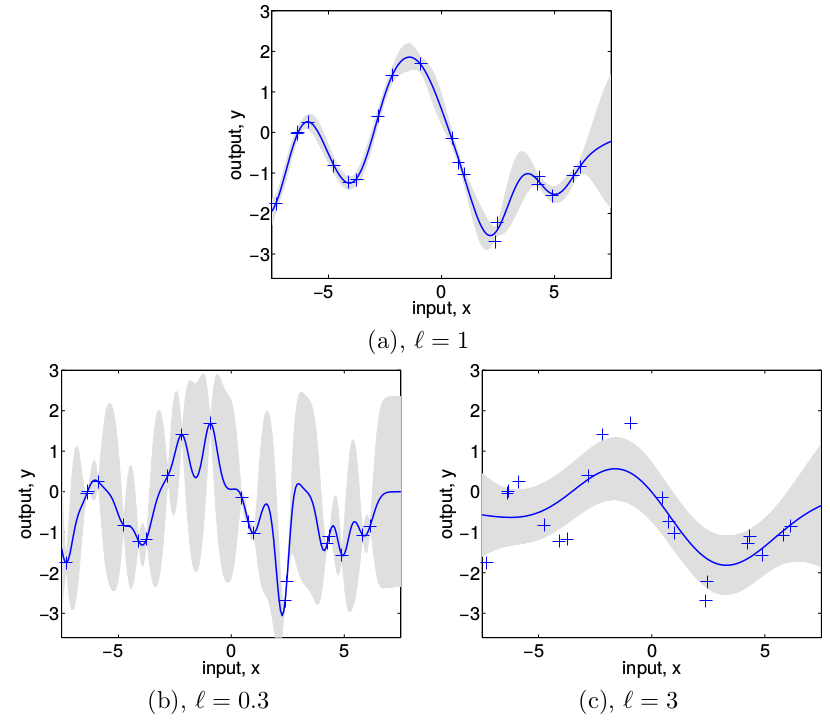
\includegraphics[scale=0.4]{rasmussen_varying_ell.png}
\caption{The effect of varying the length scale $\ell$, where the blue $+$ are data points, the blue line is the mean prediction, and the gray area is the uncertainty. Setting $\ell = 0.3$ gives a function that varies too quickly, and $\ell = 3$ is so slowly varying that it interprets much of the signal as noise. Choosing $\ell =1 $ gives the best fit to the values in this case. Figure from \cite{rasmussen2006gaussian}.}
\end{figure}

The SE is implemented in \verb|scikit-learn| under the name radial basis function, and may be called in the following way for length scale $10$, with bounds on the length scale $[0.01, 100]$
\begin{lstlisting}
from sklearn.gaussian_process.kernels import RBF
rbf = RBF(length_scale=10, length_scale_bounds=(1e-2, 1e2))
\end{lstlisting}



\subsection{The Mat\'{e}rn Kernel}

The \textit{Mat\'{e}rn class of covariance functions} is given by
\begin{align}
k_{Mat\acute{e}rn} (r) = \frac{2^{1- \nu}}{\Gamma (\nu)} \Big( \frac{\sqrt{2 \nu} r	}{\ell} \Big)^{\nu} K_{\nu} \Big( \frac{\sqrt{2 \nu}r}{\ell} \Big),
\end{align}
where $\nu, \ell > 0$, and $K_{\nu}$ is a modified Bessel function. For $\nu \rightarrow \infty$ this becomes the SE. In the case of $\nu$ being half integer, $\nu = p + \frac{1}{2}$, the covariance function is simply the product of an exponential and a polynomial
\begin{align}
k_{\nu=p+\frac{1}{2}} = \exp \Big(- \frac{\sqrt{2 \nu} r	}{\ell} \Big) \frac{\Gamma(p+1)}{\Gamma(2p + 1)} \sum^p_{i=0} \frac{(p+i)!}{i!(p-i)!} \Big( \frac{\sqrt{8 \nu} r	}{\ell} \Big)^{p-i}.
\end{align}
In machine learning the two most common cases are for $\nu = 3/2$ and $\nu = 5/2$
\begin{align}
k_{\nu = 3/2}(r) &=  \Big(1 + \frac{\sqrt{3}r}{\ell} \Big) \exp \Big( -\frac{\sqrt{3}r}{\ell} \Big),\\
k_{\nu = 5/2}(r) &=  \Big(1 + \frac{\sqrt{5}r}{\ell}  + \frac{5r^2}{3 \ell^2}\Big) \exp \Big( -\frac{\sqrt{5}r}{\ell} \Big).
\end{align}

The Mat\'{e}rn kernel is considered more appropriate for physical processes \cite{rasmussen2006gaussian}, and may be called in \verb|scikit-learn| in the following way for length scale 10, length scale bounds $[0.01, 100]$ and $\nu = 3/2$
\begin{lstlisting}
from sklearn.gaussian_process.kernels import Matern
matern = Matern(length_scale=10, length_scale_bounds=(1e-2, 1e2), nu=1.5)
\end{lstlisting}

\subsubsection{Other Kernels}

There are other kernels, but they are not introduced here. Kernels can be multiplied and summed to form new kernels, making the space of possible kernels infinite. For further details see chapter 4 in \cite{rasmussen2006gaussian}.





\subsubsection{Hyperparameters}

Each kernel has a vector of hyperparameters, e.g. $\boldsymbol{\theta} = (\{M\}, \sigma^2_f, \sigma_n^2)$ for the radial basis function (RBF)
\begin{align}
k(\textbf{x}_p, \textbf{x}_q) = \sigma_f^2 \exp (- \frac{1}{2} (\textbf{x}_p - \textbf{x}_q))^T M (\textbf{x}_p - \textbf{x}_q) + \sigma_n^2 \delta_{pq}.
\end{align}
The matrix $M$ can have several forms, for example
\begin{align}
M_1 = \ell^{-2} \mathbb{I} , M_2 = \text{diag}(\vec{\ell})^{-2}.
\end{align}
Choosing $\vec{\ell}$ to be a vector in stead of a scalar can in many cases be useful, especially if the vector of features contain values of different scales, e.g. $\textbf{x} = (x_1, x_2)$ where $x_1 \in [0, 1]$ and $x_2 \in [200, 3000]$. The length scale can be set to a vector in \verb|scikit-learn| by giving the \verb|length_scale| parameter as a \verb|numpy| array of the same dimension as the feature vector $\textbf{x}$.



\section{Model Selection}

It becomes apparent that the choice of kernel and hyperparameters is important for the quality of the GP prediction. In this section Bayesian model selection is quickly overviewed, and the log marginal likelihood and cross validation are considered for their ability to optimize the GP.

\subsection{Bayesian Model Selection}

Feature selection at several levels: posterior over \textit{parameters}, posterior over \textit{hyperparameters} and posterior for the \textit{model},
\begin{align}
p(\textbf{w}| \textbf{y}, X, \boldsymbol{\theta}, \mathcal{H}_i) = \frac{p(\textbf{y} | X, \textbf{w}, \mathcal{H}_i) p(\textbf{w}|\boldsymbol{\theta}, \mathcal{H}_i)}{p(\textbf{y}|X, \boldsymbol{\theta}, \mathcal{H}_i)}
\end{align}
\begin{align}
&p(\textbf{y}|X, \boldsymbol{\theta}, \mathcal{H}_i) = \int p(\textbf{y} | X, \textbf{w}, \mathcal{H}_i)p(\textbf{w}| \boldsymbol{\theta}, \mathcal{H}_i) d \textbf{w} & \text{(marginal likelihood)}
\end{align}
\begin{align}
p( \boldsymbol{\theta}| \textbf{y}, X, \mathcal{H}_i) = \frac{p(\textbf{y} | X, \boldsymbol{\theta}, \mathcal{H}_i) p(\boldsymbol{\theta}| \mathcal{H}_i)}{p(\textbf{y}|X,  \mathcal{H}_i)}
\end{align}
\begin{align}
p(\mathcal{H}_i| \textbf{y}, X) = \frac{p(\textbf{y} | X, \mathcal{H}_i) p( \mathcal{H}_i)}{p(\textbf{y}|X)}
\end{align}

\subsection{Log Marginal Likelihood}

For Gaussian Processes with Gaussian we can find the exact expression for the marginal likelihood,
\begin{align}
\log p(\textbf{y}|X, \boldsymbol{\theta}) = - \frac{1}{2} \textbf{y}^T K_y^{-1} \textbf{y} - \frac{1}{2} \log |K_y| - \frac{n}{2} \log 2 \pi.
\end{align}
The optimal parameters are found by maximizing the marginal likelihood
\begin{align}
\frac{\partial}{\partial \theta_j}
 \log p(\textbf{y}|X, \boldsymbol{\theta}) = \frac{1}{2} \textbf{y}^T K^{-1} \frac{\partial K}{\partial \theta_j} K^{-1} \textbf{y} - \frac{1}{2} \text{tr} (K^{-1} \frac{\partial K}{\partial \theta_j}).
\end{align}
This is what SciKitLearn uses, but can have \textbf{multiple local maxima}. Plug in Fig. 

\begin{figure}
\centering
\includegraphics[scale=0.6]{/home/ingrid/Documents/Master/Programs/LML/plots/LML_two_local_maxima.pdf}
\caption{Used SciKitLearn. Several local maxima.}
\end{figure}


\subsection{Cross Validation}

Divide into $k$-subsets and use validation and test set. Requires a loss function, e.g. $R^2$. Cross validate using Scikit-Learn, get a validation plot. Over training, over fitting, under-fitting.

\begin{figure}
\centering
\includegraphics[scale=0.4]{/home/ingrid/Documents/Master/ML/Benchmarks/learningcurve.pdf}
\caption{From scikit-learn.}
\end{figure}

\begin{figure}
\centering
\includegraphics[scale=0.4]{/home/ingrid/Documents/Master/ML/Benchmarks/learningcurve_2.pdf}
\caption{From scikit-learn.}
\end{figure}




\subsection{Loss functions}

\subsubsection{Mean Relative Deviance}

The mean relative deviance is used to quantify the quality of predictions
\begin{align}
\varepsilon = \frac{y_{true} - y_{GP}}{y_{true}}
\end{align}

\subsubsection{R-Factor}


\section{Distributed Gaussian Processes}

\subsection{Limitations of Gaussian Processes}

Problem because of $(K + \sigma_n^2 \mathbb{I})^{-1}$, means inverting an $n \times n$-matrix. Training and predicting limits of $\mathcal{O}(N^3)$ and $\mathcal{O}(N^2)$. Limit = $\mathcal{O}(10^4)$. Some solutions exist, but \textbf{no prediction of variance is given with p-o-e.}

\subsection{Product-of-Experts}

Divide data between experts. "The assumption of independent GP experts leads to a
block-diagonal approximation of the kernel matrix, which
(i) allows for efficient training and predicting (ii) can be
computed efficiently (time and memory) by parallelisation" \cite{deisenroth2015distributed}.

\begin{figure}
\centering
\includegraphics[scale=0.3]{product_of_experts.png}
\caption{From \cite{deisenroth2015distributed}.}
\end{figure}

Independence assumption
\begin{align}
p(\textbf{y} | \textbf{X}, \boldsymbol{\theta}) \approx \prod_{k=1}^M p_k(\textbf{y}^{(k)} | \textbf{X}^{(k)}, \boldsymbol{\theta}) 
\end{align}
\begin{align}
\log p(\textbf{y}^{(k)}|\textbf{X}^{(k)}, \boldsymbol{\theta}) = - \frac{1}{2} \textbf{y}^{(k)} (\textbf{K}_{\psi}^{(k)} + \sigma_{\varepsilon}^2 \textbf{I})^{-1}\textbf{y}^{(k)} - \frac{1}{2} \log
 |\textbf{K}_{\psi}^{(k)} + \sigma_{\varepsilon}^2 \textbf{I} |
\end{align}


\subsection{Algorithm}

\begin{align}
\mu_*^{rbcm} &= (\sigma_*^{rbcm})^2 \sum_k \beta_k \sigma_k^{-2} (\textbf{x}_*) \mu_k (\textbf{x}_*),\\
(\sigma_*^{rbcm})^{-2} &= \sum_{k=1}^M \beta_k \sigma_k^{-2} (\textbf{x}_*) + \big(1 - \sum_{k=1}^M \beta_k \big) \sigma_{**}^{-2}.
\end{align}
The posterior distribution for the test point $\textbf{x}_*$ is given by a Gaussian with mean and variance
\begin{align}
\mu (\textbf{x}_*) &= \textbf{k}_*^T (\textbf{K} + \sigma_{\epsilon}^2 \mathbb{I})^{-1} \textbf{y},\\
\sigma^2(\textbf{x}_*) &= k_{**} - \textbf{k}_*^T(\textbf{K} + \sigma_{\epsilon}^2 \mathbb{I})^{-1} \textbf{k}_*.
\end{align}




Plot of time from the article 

\begin{figure}
\centering
\includegraphics[scale=0.4]{DGP_times.png}
\caption{From \cite{deisenroth2015distributed}.}
\end{figure}

\subsection{Implementing the Algorithm}

\begin{algorithm}
 \KwData{$N_{experts}$ (number of experts), $X$ (inputs), \textbf{y} (targets), $k$ (covariance function/kernel), $\sigma_n^2$ (noise level), $\textbf{x}^*$ (test input), $\textbf{y}^*$ (test target)}
$X_{train}$, $X_{test}$, $y_{train}$, $y_{test}$ = train-test-split $(X, y)$ (scikit-learn) \;
$y = \log_{10} (y)$ \;
$n = \frac{\text{Number of data points}}{N_{experts}}$ \;
$subsets = array\_split (X_{train}, n)$ \;
$\mu_{rbcm} = []$, $\sigma_{rbcm} = []$  (empty lists to be filled later)\; 
\For {each expert}
{
$gp_{temporary} = GaussianProcessRegressor.fit(X_{expert}, y_{expert})$ \;
 \For {each $y^*$ in $\textbf{y}^*$}
 {
 $\mu_*,\sigma_*^2 = gp_{temporary}.predict(x^*)$ \;
 $\sigma_{**}^2 = k (x^*, x^*)$ \;
 (fill inn the values) \;
 $\boldsymbol{\mu}[\text{expert}][x^*] = \mu_*^2$ (mean value from this expert)\;
 $\boldsymbol{\sigma}^2[\text{expert}][x^*] = \sigma_*^2$ (variance from this expert)\;
 $\boldsymbol{\sigma}_{**}^2[\text{expert}][x^*] = \sigma_{**}^2$ (variance from initial kernel)
 }
}
 
\For {each expert}
{ 
\For {each $y_*$ in $\textbf{y}_*$}
{ $\mu_* = \boldsymbol{\mu}[\text{expert}][x_*]$ (retrieve relevant values)\;
$\sigma_*^2 = \boldsymbol{\sigma}^2[\text{expert}][x^*]$ \;
$\sigma_{**}^2 = \boldsymbol{\sigma}_{**}^2[\text{expert}][x^*]$ \; 
$\beta = \frac{1}{2} (\log (\sigma_{**}^2) - \log (\sigma_*^2))$ \;
$(\sigma_*^{rbcm})^{-2}[y_*] += \beta \sigma^{-2} + \big(\frac{1}{n_{experts}} - \beta \big) \sigma_{**}^{-2} $ }
 }  
\For {each expert}
{
\For {each $y_*$ in $\textbf{y}_*$}
 {
$\mu_* = \boldsymbol{\mu}[\text{expert}][x_*]$ (retrieve relevant values)\;
$\sigma_*^2 = \boldsymbol{\sigma}^2[\text{expert}][x^*]$ \;
$\sigma_{**}^2 = \boldsymbol{\sigma}_{**}^2[\text{expert}][x^*]$ \; 
$\beta = \frac{1}{2} (\log (\sigma_{**}^2) - \log (\sigma_*^2))$ \;
$\mu_*^{rbcm}[y_*] += (\sigma_*^{rbcm})^2 \beta \sigma^{-2}_* \mu_*$
 }
} 
$\epsilon = \frac{10^{\mu_{rbcm}} - 10^{y_{test}}}{10^{y_{test}}}$ (relative error)\;
\KwResult{Approximative distribution of $f_* = f(\textbf{x}_*)$ with mean $\mu^{rbcm}_*$ and variance $(\sigma^{rbcm}_*)^2$.}
 \caption{Algorithm for using rBCM on a single test point $\textbf{x}_*$. The $GaussianProcessRegressor.fit()$-function is a function in scikit-learn, that uses Algorithm (\ref{Alg:: GP}). }
\label{Alg:: DGP}
\end{algorithm}

\subsubsection{Parallelizing}

\subsection{Benchmark}



\bibliographystyle{plain}
\bibliography{dingsen_gaussian_processes}



\end{document}